\documentclass{article}

\usepackage[left=1.5cm, right=1.5cm, top=3cm, bottom = 3cm]{geometry}

\usepackage{amsmath}
\usepackage{amsfonts}
\usepackage{amssymb}
\usepackage{graphicx}
\usepackage{float}
\usepackage{indentfirst}
\usepackage{wrapfig}
\usepackage{latexsym}
\usepackage{hyperref}
\usepackage{feynmf}
\linespread{1.1}

% frequently used 3-vector notations
\newcommand{\mtp}{\mathbf{p}}
\newcommand{\mtq}{\mathbf{q}}
\newcommand{\mtk}{\mathbf{k}}
\newcommand{\pnx}{\mathbf{x}}
\newcommand{\pny}{\mathbf{y}}
\newcommand{\pnr}{\mathbf{r}}

% frequently used spin notations

\newcommand{\uspin}{\uparrow}
\newcommand{\dspin}{\downarrow}

\author{Fang Xie, \emph{Department of Physics, Tsinghua University}}
\title{{\bf{An Introduction to Second Quantization in Statistical Mechanics}}}
\date{\today}

\begin{document}
\maketitle
\section{Introduction}
Second Quantization is the best way to describe the many-body quantum systems. We can use the creation-annihilation operators to get a lot of interesting results by this method. In this article I will follow the formalism of Pathria's book and show how to use second quantization to get the statistical properties of boson liquid and fermi liquid.

\section{Second quantization of Bosons and Fermions and free particle system}
\subsection{Second Quantization Algebra}
Actually second quantization is the quantization of fields. So we need to define the creation-annihilation operators of the boson or fermion field:
\begin{eqnarray}
[a_i,a^\dagger_j] &=& \delta_{ij}\\
\left[a_i,a_j\right] &=& 0 \\
\left[a^\dagger_i,a^\dagger_j\right] &=& 0 
\end{eqnarray}
and the vacuum state is needed: $|0\rangle$. We can act the creation operator on the vacuum state to obtain a single-particle state. And the subspace (of the Hilbert space) with different particle numbers are connected by these operators. See the figure below:
\begin{figure}[!htp]
\centering
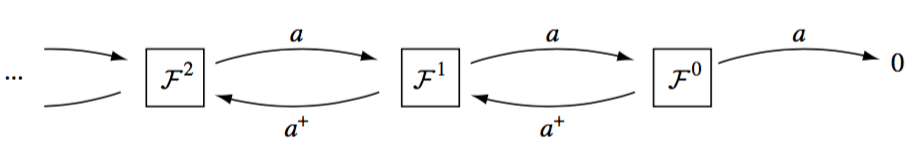
\includegraphics[width=10cm]{./figure/pic1.png}
\caption{Fock space}
\end{figure}

In Eq.(1)(2)(3), indexes $i,j$ means some eigenvalue of some operators. For Fermions the commutation relation is altered by anti-commutation relation. Since the commutation relation is just like the upper and lower operators of Harmonic oscillator, we can find that
$$
N = \sum_i a^\dagger_i a_i 
$$
is the operator of particle number. For example we can find that the normalized $N$ particle state can be written as:
$$
|\psi\rangle = \prod_{i}\frac{1}{\sqrt{n_i !}}a^\dagger_i |0\rangle
$$
\subsection{One-body Operators}
Now introduce the {\bf{one-body operator}}: for any one-body operator $\mathcal{O}_1$, its second-quantized form under its eigenbasis are:
\begin{equation}
\hat{O} = \sum_{i}o_i a^\dagger_i a_i
\end{equation}
and $o_i$ is the eigenvalue of first-quantized operator $O_1$. Now if we do an representation transformation to basis that are not the eigenvectors of $O_1$, then the operators will change into:
\begin{equation}
a^\dagger_{i'} = \sum_i \langle i | i'\rangle a^\dagger_i
\end{equation}
then the second quantized operator will be:
\begin{equation}
\hat{O} = \sum_{ij}\langle i | O_1|j\rangle\, a^\dagger_i a_j
\end{equation}
For example, the second quantized Hamiltonian is
$$
H = \sum_{\mtk\sigma}\epsilon_{\mtk}a^\dagger_{\mtk\sigma}a_{\mtk\sigma} \quad\textrm{Free particle system}
$$
or
$$
H = -t\sum_{\langle ij \rangle}a^\dagger_i a_j\quad \textrm{(Tight-binding approximation)}
$$
Now if we transform to the real-space representation, the Hamiltonian will have the following form:
\begin{equation}
H = \int d^3x\,\psi^\dagger(\pnx)\left(-\frac{\hbar^2}{2m}\nabla^2\right)\psi(\pnx)
\end{equation}
in which $\psi^\dagger(\pnx)$ is the creation operator at position $\pnx$. This is easily obtained from Eq.(6).

\section{Relation between first quantization and second quantization}
\subsection{Wave Function}
So what is the relationship between the formalism with so called ``first quantization'' we familiar with? Remember that the wave function is the inner product of $\langle \pnr_i|$ (the eigenvector of the position operator) and the eigenstate of the Hamiltonian $|\psi\rangle$ (with fixed particle number $N$), we can find that
\begin{equation}
\psi_{N}(\pnr_i) = \langle \pnr_i | \psi_N\rangle = \frac{1}{\sqrt{N!}}\langle 0| \psi(\pnr_1) \psi(\pnr_2)\cdots \psi(\pnr_N)|\psi_N\rangle
\end{equation}
and it automatically satisfies the exchange symmetry of Boson wave function. We can also find that this wave function is normalized:
\begin{eqnarray}
\int d^{3N}r\,\psi(\pnr_i)\psi^*(\pnr_i) &=& \frac{1}{N!}\int d^{3N}r\,\langle \psi_N | \psi^\dagger(\pnr_N)\cdots\psi^\dagger(\pnr_1)|0\rangle \langle 0|\psi(\pnr_1)\cdots \psi(\pnr_N)|\psi\rangle\nonumber\\
&=& \frac{1}{N!}\int d^{3N}r \, \langle \psi_N |\psi^\dagger(\pnr_N)\cdots \psi^\dagger(\pnr_1)\psi(\pnr_1)\cdots \psi(\pnr_N)|\psi_N\rangle\nonumber\\
&=&\frac{1}{N!} \int d^{3N-3}r \, \langle \psi_N|\psi^\dagger(\pnr_N) \cdots\psi^\dagger(\pnr_2)N\psi(\pnr_2)\cdots \psi^(\pnr_N)|\psi_N\rangle \nonumber\\
&=& \frac{1}{N!} \int d^{3N-6}r \, \langle \psi_N|\psi^\dagger(\pnr_N) \cdots\psi^\dagger(\pnr_3)N(N-1)\psi(\pnr_3)\cdots \psi^(\pnr_N)|\psi_N\rangle \nonumber\\
&=& \frac{1}{N!}\langle \psi_N| N(N-1)\cdots |\psi_N\rangle\nonumber\\
&=& 1
\end{eqnarray}
So clearly we see that the wave function is the inner product of a position eigenstate and an quantum state with a fixed particle number.

\subsection{Schr$\ddot{\mathbf{o}}$dinger Equation}
In this part I will show that the wave function we get in the previous section satisfies the Schr$\ddot{\textrm{o}}$dinger equation. Now assume that the quantum state $|\psi_N\rangle$ has fixed particle number and energy, and we calculate the following equation:
\begin{eqnarray}
E_N\psi_N(\pnr) &=& \frac{1}{\sqrt{N!}}\langle 0| \psi(\pnr_1)\cdots  \psi(\pnr_N) H |\psi_N\rangle\nonumber\\
&=& \frac{1}{\sqrt{N!}}\langle 0| \sum_{i=1}^N  \int d^3 \pnr\,\psi(\pnr_1)\cdots \psi(\pnr_{i-1})\delta(\pnr-\pnr_i) \psi(\pnr_{i+1})\cdots  \psi(\pnr_N)\left(-\frac{\hbar^2\nabla^2}{2m}\right)\psi(\pnr)|\psi_N\rangle\nonumber\\
&=& \frac{1}{\sqrt{N!}}\sum_{i=1}^N (-\frac{\hbar^2\nabla_i^2}{2m})\langle 0| \psi(\pnr_1)\cdots  \psi(\pnr_N)|\psi_N\rangle \nonumber\\
&=& \sum_{i=1}^N (-\frac{\hbar^2\nabla_i^2}{2m})\psi_N(\pnr)
\end{eqnarray}
So up till now we have proved that the wave function satisfies the Schr$\ddot{\textrm{o}}$dinger equation. The interacting term is the same, and for simplicity, I won't show it here. 

\section{Interacting Boson system}
\subsection{Two-body interaction term}
Now we need to add the interaction term into the Hamiltonian. In the momentum representation, the Hamiltonian will be:
\begin{equation}
H=\sum_{\mtk\sigma}\frac{\mtk^2}{2m}a^\dagger_{\mtk\sigma}a_{\mtk\sigma} + \frac{1}{2L^3}\sum_{\mtk\mtk'\mtq}u_\mtq a^\dagger_{\mtk+\mtq\sigma}a^\dagger_{\mtk'-\mtq\sigma'}a_{\mtk'\sigma'}a_{\mtk\sigma}
\end{equation}
And this can be easily obtained from the Fourier transformation of an interacting system:
$$
\hat{u} = \frac{1}{2}\int d^3x d^3 x'\, V(\pnx-\pnx')\rho(x)\rho(x')\,.
$$
and the interacting term can be shown by the following graph:
\begin{figure}[!htp]
\centering
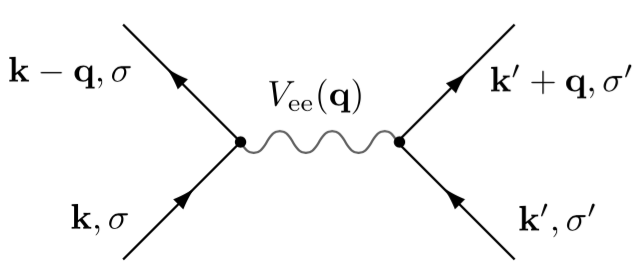
\includegraphics[width = 7cm]{./figure/pic2.png}
\caption{``Feynman Diagram''}
\end{figure}\\
Now if we write the interacting term by the scattering length, the Fourier component will be 
$$
a(\mtq) = 
$$

\section{Low temperature behavior of imperfect Bose gas}

\section{Vortex and Topological Excitations}

\end{document}